%! TeX root = ../autoref.tex

\noindent
{\Large Автореферат ВКР}

\noindent
\textbf{Тема работы}: Метод компенсации нелинейных искажений усилителя
мощности для стандарта мобильной связи 5G NR

\noindent
\textbf{Выполнил}: Шиков А.П., Магистратура, 2 курс, Радиофизический факультет

\subsection*{Введение и актуальность}
Развитие стандарта мобильной связи 5G NR тесно связано с технологией
Интернета Вещей. Система имеет необходимую надежность и скорость передачи,
что важно для эффективной работы системы. Помимо этого ведутся активные
работы по расширению рабочего диапазона частот до 114 ГГц, что позволит еще
больше увеличить пропускную способность.
% Высокая скорость, надежность сети, малая задержка, а также возможность
% массового подключения "умных" устройств являются важнейшими параметрами,
% определяющими производительность системы в целом.
Однако в этом диапазоне появляется ограничение в виде нелинейных искажений,
вызванных работой усилителя мощности (УМ). Несмотря на продвижение в
технологии разработки и проектирования УМ, все еще наблюдаются значительные
искажения сигнала при стандартной мощности передатчика.

Проблема наиболее актуальна при применении стандарта 5G к технологии
Интернета Вещей. В данном случае система имеет множество простых передающих
устройств, таких как датчики и сенсоры. Элементы часто имеют
низкокачественные передающие и усилительные цепи для снижения общей
стоимости прибора, устройства также должны минимизировать общее потребление
электроэнергии. Эти факторы являются ключевыми при выборе метода
компенсации искажений, поскольку обработка на передатчике может внести
дополнительные энергозатраты.

Основными целями работы являются исследование влияния нелинейности
усилителя мощности на различные типы сигнала, используемые в стандарте 5G,
разработка модели усилителя для миллиметрового диапазона 100-200 ГГц, а
также разработка метода компенсации нелинейных искажений усилителя мощности
на приемнике.

\subsection*{Содержание работы}
В работе изучается влияние нелинейности УМ на производительность
системы. Для описания работы усилителя использовалась модель Раппа для
диапазона 30-70 ГГц. Также была разработана усредненная модель для
диапазона 100-200 ГГц. 

Использование нелинейного УМ приводит к значительным искажениям сигналов
CP-OFDM и DFT-s-OFDM. В результате при декодировании принятого сигнала
возникают ошибки, понижающие эффективность работы системы. При
использовании модели 100-200 ГГц искажения носят более сильный характер.
Возникает необходимость компенсации внесенных искажений. Обработка возможна
на передатчике или приемнике, однако для минимизации нагрузки на передающее
устройство использование компенсации на приемнике предпочтительнее.

В работе описывается новый метод компенсации нелинейных искажений внесенных
усилителем мощности на приемнике для двух типов сигнала - CP-OFDM и
DFT-s-OFDM. Основа метода заключается в применении обработки, эквивалентной
обработке на передатчике для переноса сигнала во временную область, где
сигнал искажался усилителем, а также применении ограниченной обратной
амплитудной характеристики усилителя на основе известных параметров для
компенсации искажений. Рассматривается применение метода для различных
типов сигнала.

\subsection*{Результаты}
Усилитель и разработанный метод компенсации были реализованы в симуляторе
канального уровня. В работе описываются результаты моделирования системы
при различных параметрах (тип сигнала, модель усилителя, SCS, модуляция и
другие) для оценки влияния нелинейности усилителя и эффективности
предложенного метода. Пример полученных результатов для модели 30-70 ГГц
приведен на рис. \ref{fig:res3070_scs120} и для модели 100-200 ГГц на рис.
\ref{fig:res100200_scs120}.
\begin{figure}[h!]
    \centering
    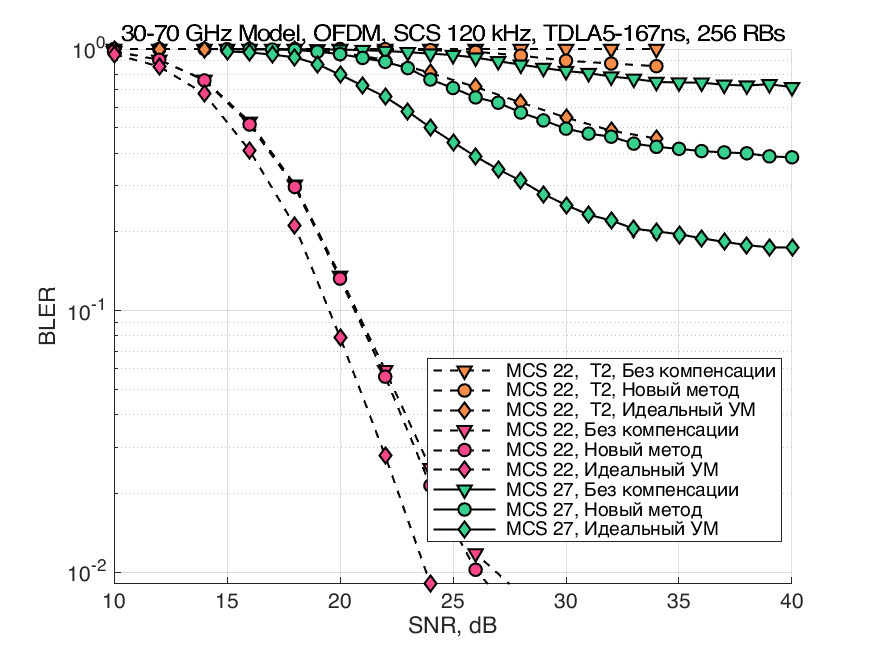
\includegraphics[width=0.49\linewidth]{figs/res/ofdm/OFDM_Nokia_SCS120_MCS22_27.png}
    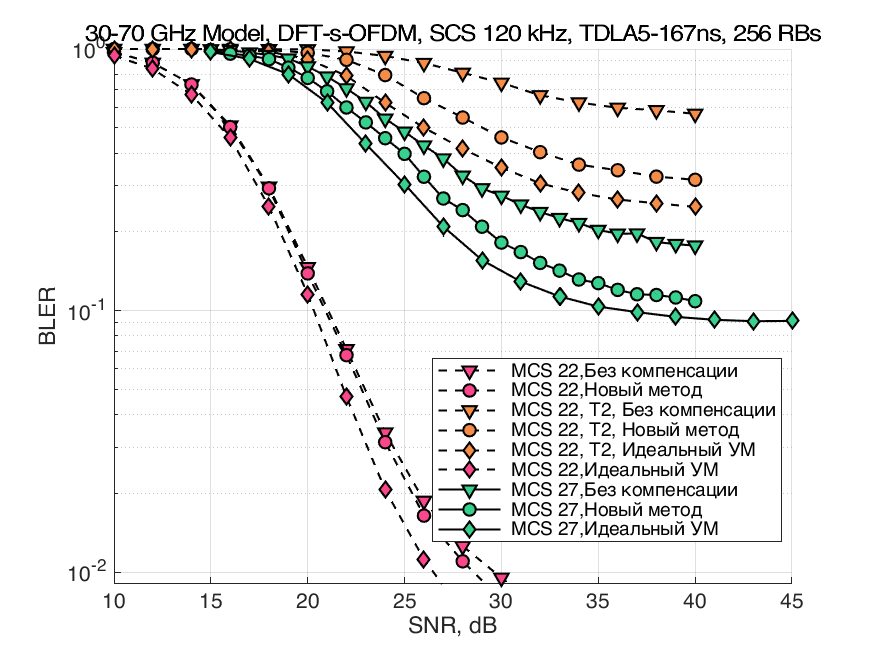
\includegraphics[width=0.49\linewidth]{figs/res/dftsofdm/DFT-s-OFDM_Nokia_SCS120_MCS22_27.png}
    \caption{BLER для SCS 120 кГц, 64-QAM/256 QAM для OFDM (слева) для DFT-s-OFDM(справа)}
    \label{fig:res3070_scs120}
\end{figure}

\begin{figure}[h!]
    \centering
    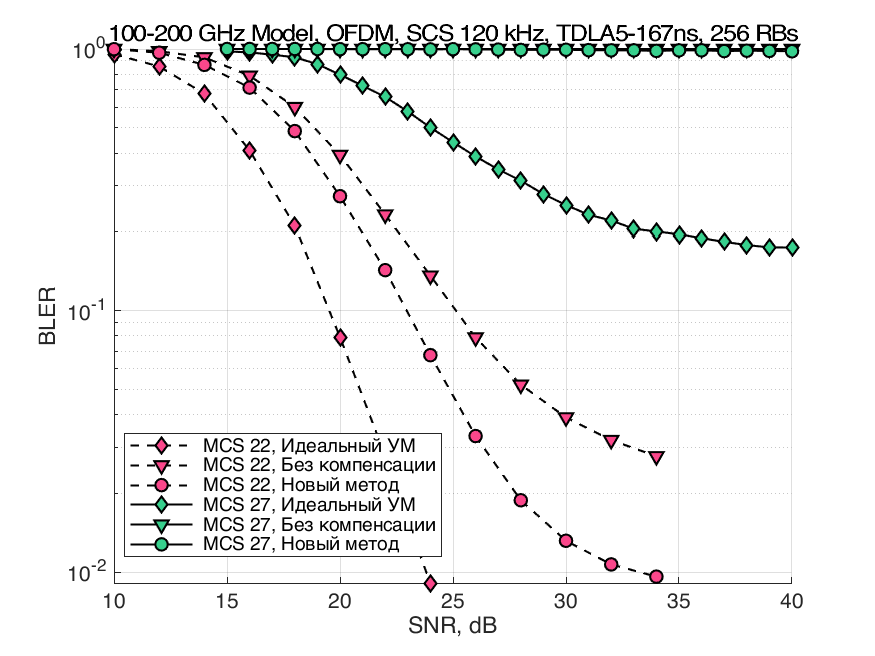
\includegraphics[width=0.49\linewidth]{figs/res/ofdm/OFDM_SubTHz_SCS120_MCS22_27.png}
    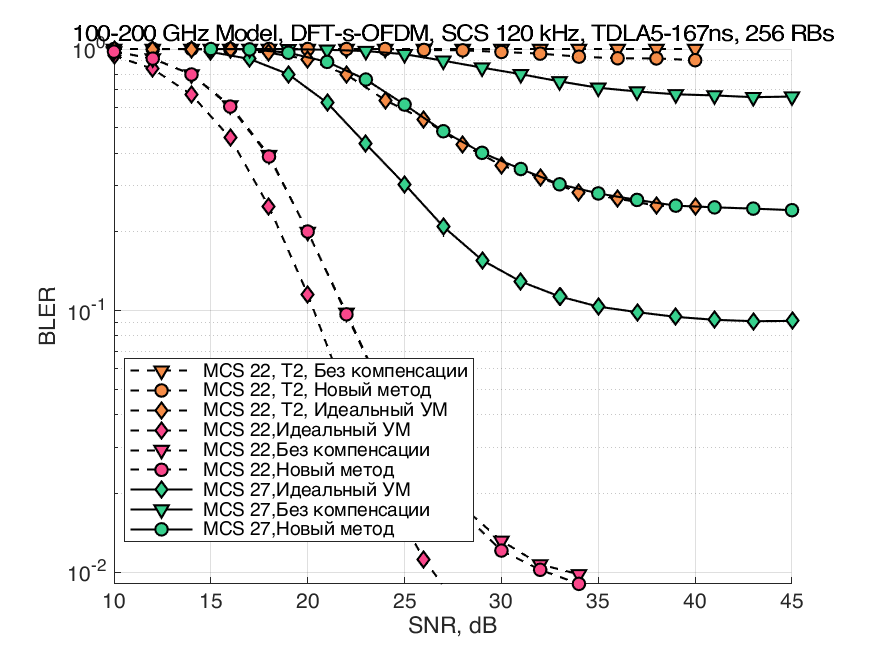
\includegraphics[width=0.49\linewidth]{figs/res/dftsofdm/DFT-s-OFDM_SubTHz_SCS120_MCS22_27.png}
    \caption{BLER для SCS 120 кГц, 64-QAM/256 QAM для OFDM (слева) для DFT-s-OFDM(справа)}
    \label{fig:res100200_scs120}
\end{figure}
% Для модели УМ в диапазоне 30-70 ГГц улучшение наблюдается в основном только
% для модуляций высокого порядка и при высоких значениях SCS. Однако можно
% наблюдать улучшение результатов — кривые BLER в случае компенсации
% смещаются на несколько dB по сравнению со случаем отсутствия компенсации.
% Для модели 100-200 ГГц, влияние нелинейности увеличивается, что связано
% с общим ухудшением характеристик усилителя в данном диапазоне. В некоторых
% случаях, искажения настолько сильные, что восстановление информации
% практически невозможно.

Предложенный метод компенсации демонстрирует улучшение результата как для
сигнала DFT-s-OFDM, так и для сигнала CP-OFDM. В большинстве случаев, при
отсутствии эффекта насыщения кривой BLER, разработанный метод улучшает
результат на несколько dB. Например, для сигнала OFDM SCS 120 кГц при MCS
22 рис. (\ref{fig:res100200_scs120}), компенсация улучшила результат на 2-3
dB.

Разработанный метод компенсирует искажения на стороне приемника, такой подход
эффективен в системе с большим количеством простых, дешевых передатчиков с
низким энергопотреблением, такой как инфраструктура IoT. Это позволит
устройству передачи снизить общее потребление энергии, поскольку
отсутствует необходимость в предварительной обработке сигнала на
передатчике.

В работе было изучено влияние искажений нелинейного усилителя на
эффективность работы системы. Так же была разработана модель усилителя для
диапазона 100-200 ГГц. Описан и протестирован метод компенсации искажений
на приемнике, адаптируемый в зависимости от используемого сигнала. Метод
продемонстрировал возможность улучшить результат работы системы для числа
случаев, основное преимущество метода заключается в обработке на приемнике,
что минимизирует нагрузку на передатчик.